\chapter{Syntaktická analýza}
Syntaktickou analýzou (slangovo z angličtiny tiež \textbf{parsovaním}) sa v teórii rozumie konštrukcia derivačného stromu vety bezkontextového jazyka\cite{CVUT:program_language} popísaného v kapitole \ref{CFG}. Program, ktorý vykonáva túto úlohu sa volá syntaktický analyzátor (slangovo \textbf{parser}). Počas konštrukcie derivačného stromu parser zachováva hierarchické usporiadanie symbolov, ktoré je vhodné pre ďalšie spracovanie.

Parsovanie je taktiež možné si predstaviť ako inverziu k napĺňaniu šablón. Šablóna definuje napríklad štruktúru textu s variabilnými premennými, ktoré je potrebné naplniť dátami a parsovanie identifikuje túto šablónu a extrahuje dáta, ktoré boli do nej vložené.

\begin{figure}[H]
\begin{center}
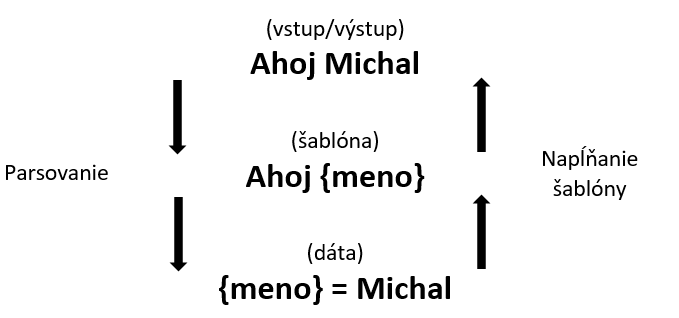
\includegraphics[width=10cm]{figures/templatingAndParsing.PNG}
\caption{Príklad parsovania a napĺňania šablóny}
\label{fig:templatingAndParsing}
\end{center}
\end{figure}

Podstata parsovania je veľmi dôležitá, pretože rôzne entity potrebujú dáta na spracovanie v rôznych formátoch. Parsovanie umožňuje transformovať získané dáta tak, aby im mohol porozumieť špecifický software. 

\section{Teória parsovania}
Na správne pochopenie problému parsovania je nutné najprv zadefinovať základné pojmy, ktoré sú s ním spojené. Teória parsovania je postavená na teórii jazykov, gramatík a automatov, z ktorej najdôležitejšie pojmy sú definované v rámci tejto sekcie.

\subsection{Deterministický konečný automat}\label{DFA}
Konečné automaty sa používajú v rôznych oboroch ako napríklad pri prekladačoch, spracúvaní prirodzeného jazyka, pri návrhu hardwaru a ďalších \cite{demlova:automaty}. Predstavujú model systémov, ktoré rozpoznajú, či vstupný reťazec patrí do jazyka. Deterministický konečný automat (\nom{DFA}{Deterministic Finite Automaton}), taktiež aj \textit{akceptor}, je najpoužívanejší zo štyroch typov automatov.

\begin{definice}
\textit{Deterministický konečný automat} $M$ je pätica $M = (Q,\Sigma,\delta, q_0, F)$, kde
\begin{itemize}
\item $Q$ je konečná množina stavov
\item $\Sigma$ je konečná množina vstupných symbolov
\item $\delta$ je prechodová funkcia $\delta: Q \times \Sigma \rightarrow Q$
\item $q_0$ je počiatočný stav
\item $F \subseteq Q$ je množina koncových stavov \cite{demlova:automaty}
\end{itemize}
\end{definice}

Konečný automat je možné prehľadne znázorniť formou stavového diagramu. \textit{Stavový diagram} je orientovaný graf, v ktorom sú uzly ohodnotené stavmi automatu a hrany vstupnými symbolmi automatu. Z uzlu $q$ vedie hrana ohodnotená symbolom $a$ do uzlu $p$ vtedy, ak $\delta(q,a) = p$. Počiatočný stav sa označuje šípkou, ktorá neprichádza zo žiadneho iného stavu a uzly ohodnotené koncovými stavmi označujeme dvojitým krúžkom. Príklad takto znázorneného DFA je na obrázku \ref{fig:DFA_example}.

\begin{figure}[H]
\begin{center}
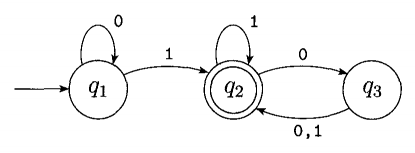
\includegraphics[width=8cm]{figures/DFA_example.PNG}
\caption{Príklad DFA znázorneného pomocou stavového diagramu}
\label{fig:DFA_example}
\end{center}
\end{figure}

\begin{definice}[\textbf{Jazyk prijímaný konečným automatom}]\label{def:regular_language}
Je daný DFA $M = (Q,\Sigma,\delta, q_0, F)$. Slovo $u \in \Sigma^*$ je \textit{prijímané} automatom $M$ práve vtedy, keď
\begin{center}
$\delta^*(q_0,u) \in F$.
\end{center}
Množina všetkých slov, ktoré automat prijíma sa nazýva \textit{jazyk prijímaný} $M$ a značíme ju $L(M)$. Platí teda
\begin{center}
$L(M) = \{\omega|\delta^*(q_0,u) \in F\}$.\cite{demlova:automaty}
\end{center}
\end{definice}

Každý jazyk $L$, pre ktorý existuje deterministický konečný automat prijímajúci tento jazyk, sa nazýva \textbf{regulárny jazyk}.

\subsection{Regulárny výraz}\label{regexp}
Regulárny výraz je ďalšia možnosť, ako popísať regulárne jazyky, ktoré sú uzatvorené vzhľadom k operáciám zjednotenia, súčinu a iterácie. Regulárne výrazy sú postavené na Kleeneho operátore(*), ktorý sa používa na označenie, že určitý prvok môže byť prítomný nula alebo nekonečne veľa krát.
\begin{definice}[\textbf{Regulárne výrazy nad abecedou}]
Je daná abeceda $\Sigma$. Množina všetkých regulárnych výrazov nad $\Sigma$ je definovaná induktívne:
\begin{itemize}
\item $\emptyset$ je regulárny výraz,
\item $\epsilon$ je regulárny výraz,
\item \textbf{a} je regulárny výraz pre každé písmeno $a \in \Sigma$,
\item pokiaľ sú \textbf{r$_1$} a \textbf{r$_2$} regulárne výrazy, tak \textbf{r$_1$ + r$_2$}, \textbf{r$_1$r$_2$} a \textbf{r$_1^*$} sú regulárne výrazy. \cite{demlova:automaty}
\end{itemize}
\end{definice}

Podpora regulárnych výrazov je dostupná u väčšiny programovacích jazykov. Pre zjednodušenie zápisu sú definované viaceré znaky, ktoré vychádzajú zo spomenutých základných operácií. Ich najčastejšie využitie je na vyhľadávanie v texte.

% You can implement a lexer using the regular expression engine provided by your language. However usually the regular expressions defined in the grammar are converted are actually converted to a finite-state machine to gain better performance.

\subsection{Bezkontextový jazyk}\label{CFG}
Bezkontextový jazyk je jazyk nad abecedou, ktorý je prijímaný bezkontextovou gramatikou (\nom{CFG}{context-free grammar}). Gramatikou sa rozumie súpis pravidiel, ktoré určujú ako vygenerovať všetky slová daného jazyka. CFG reprezentuje silnejšiu metódu popisovania jazykov, pomocou ktorej je možné opísať vlastnosti, ktoré majú rekurzívnu štruktúru.

\begin{definice}
\textit{Bezkontextová gramatika} je usporiadaná štvorica $\mathcal{G} = (N, \Sigma , S, P)$, kde
\begin{itemize}
\item $N$ je konečná množina tzv. \textit{neterminálov}\footnote{Premenné symboly, ktoré sa reprezentjú pomocou velkých písmen}
\item $\Sigma$ je konečná neprázdna množina tzv. \textit{terminálov}\footnote{Písmená vstupnej abecedy, často reprezentované malými písmenami, číslami alebo špeciálnymi symbolmi}, kde platí $N \cap \Sigma = \emptyset$
\item $S \in N$ je \textit{štartovací symbol}
\item $P$ je konečná množina pravidiel typu $\alpha \rightarrow \beta$, kde $\alpha$ a $\beta$ sú slová nad $N \cup \Sigma$ taká, že $\alpha$ obsahuje aspoň jeden neterminál. 
\item každé pravidlo $P$ je v tvare $A \rightarrow \gamma$, kde $\gamma \in (n \cup \Sigma)*$ a $A$ je neterminál \cite{demlova:gramatiky}
\end{itemize}
\end{definice}

Bezkontextové gramatiky sa prvýkrát používali pri štúdiu ľudských jazykov na pochopenie vzťahu medzi podstatným menom, slovesom a predložkou. Ich kombináciou vznikajú frázy, ktoré vedú k prirodzenej rekurzii, nakoľko podstatné meno môže byť súčasťou slovesnej frázy a pod. Bezkontextové gramatiky dokážu zachytiť dôležité aspekty týchto vzťahov \cite{computation_theory}.

Špecifikácia a kompilácia programovacích jazykov je jedným z použití CFG. Gramatika programovacieho jazyka sa často používa na pochopenie jeho syntaxe.

V nasledujúcom príklade je ukážka bezkontextovej gramatiky $G_1$.
\begin{center}
\begin{tabular}{p{0.12\textwidth}}
$A \rightarrow 0A1$\\
$A \rightarrow B$\\
$B \rightarrow $\#
\end{tabular}
\end{center}

Z týchto pravidiel je možné poskladať strom pravidiel, v ktorom je množina terminálov $\Sigma \in \{0,1,\#\}$, množina neterminálov $N \in \{A, B\}$ a štartovací symbol je $A$. 

\begin{definice}[\textbf{Derivácia}]
Je daná gramatika $\mathcal{G} = (N, \Sigma , S, P)$. Povedzme, že $\delta$ sa \textit{odvodí} z $\gamma$ vtedy, ak
\begin{itemize}
\item buď $\gamma = \delta$
\item alebo existuje postupnosť priamych odvodení
\end{itemize}
\begin{center}
$\gamma = \gamma_1 \Rightarrow_\mathcal{G} \gamma_2 \Rightarrow_\mathcal{G} ... \Rightarrow_\mathcal{G} \gamma_k = \delta$
\end{center}
Tento fakt sa označuje $\gamma\Rightarrow_\mathcal{G}^*\delta$ a tejto konečnej postupnosti hovoríme \textit{derivácia}. \cite{demlova:gramatiky}
\end{definice}

Pre príklad, gramatika $G_1$ generuje  reťazec \textit{000\#111}. Derivácia tohto reťazca bude vyzerať nasledovne
\begin{center}
$A \Rightarrow 0A1 \Rightarrow 00A11 \Rightarrow 000A111 \Rightarrow 000B111 \Rightarrow 000\#111$
\end{center}

Rovnakú informáciu je možné reprezentovať graficky pomocou zparsovaného (derivačného) stromu. Príklad derivačného stromu je na obrázku \ref{fig:derivacni_strom}. 

\begin{figure}[H]
\begin{center}
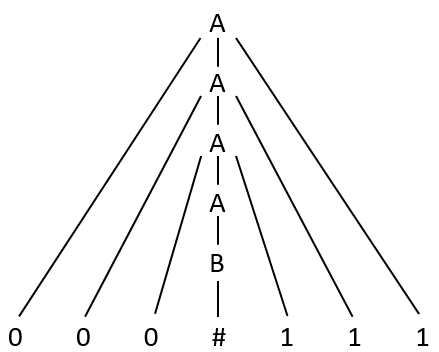
\includegraphics[width=5cm]{figures/derivacni_strom.PNG}
\caption{Derivačný strom gramatiky $\mathcal{G}_1$ pre reťazec \textit{000\#111}}
\label{fig:derivacni_strom}
\end{center}
\end{figure}

Množina všetkých reťazcov, ktoré je možné generovať týmto spôsobom sa nazýva jazyk gramatiky $L$. Jednoduchým pohľadom na gramatiku $G_1$ je možné zapísať jazyk gramatiky ako $L(G_1) \in \{0^n\#1^n | n \geq 0\}$. Všetky jazyky generované bezkontextovou gramatikou sa nazývajú \textbf{bezkontextové jazyky}.

\begin{definice}[\textbf{Jazyk generovaný gramatikou}]
Povedzme, že slovo $\omega \in \Sigma^*$ je \textit{generované} gramatikou $\mathcal{G}$, ak existuje derivácia $S\Rightarrow_\mathcal{G}^*\omega$.

\textit{Jazyk $L(\mathcal{G})$ generovaný} gramatikou $\mathcal{G}$ sa skladá zo všetkých slov generovaných gramatikou $\mathcal{G}$, tj.
\begin{center}
$L(\mathcal{G}) = \{\omega \in \Sigma^* | S \Rightarrow_\mathcal{G}^* \omega\}$.\cite{demlova:gramatiky}
\end{center}
\end{definice}

\subsection{Backus-Naur Form notácia}\label{BNF}
Pri popisovaní jazyka mnohých programovacích jazykov, protokolov alebo formátov sa vo svojej špecifikácii používa zápis pomocou Backus-Naur Form (\nom{BNF}{Backus-Naur Form}) notácie.\cite{might:languages} 

Každé pravidlo v BNF má nasledujúcu štruktúru:
\begin{center}
\textit{<neterminál> ::= výraz}
\end{center}

Všetky netreminály v BNF sa zapisujú do špicatých zátvoriek \textit{< >}, či už sú použité na pravej alebo ľavej strane pravidla. Výraz sa môže obsahovať terminály aj neterminály a je definovaný ich spojením alebo výberom. Symboly vo výraze postavené vedľa seba určujú postupnosť symbolov a použitie znaku vertikálnej lišty určuje výber zo symbolov.

\subsection{Rozšírená Backus-Naur Form notácia}\label{EBNF}
Pre zjednodušenie zápisu gramatiky a aby bolo možné jednoduchšie definovať určité typy pravidiel, vznikla kolekcia rozšírení k Backus-Naur Form notácii (\nom{EBNF}{Extended Backus-Naur Form}), ktorá bola štandardizovaná ako ISO/IEC 14997\cite{ISO14977}. Terminály môžu byť vyjadrené konkrétnym postupom znakov v úvodzovkách alebo pomocou triedy literálov, ktorú je možné zapísať pomocou regulárneho výrazu. Priraďovací znak pravidla je zmenený z ::= na jednoduché = a vynecháva sa zápis špicatých zátvoriek okolo neterminálov. Tieto malé syntaktické zmeny nie sú tak dôležité ako dodatočné operácie EBNF, ktoré sa môžu použiť vo výraze.

\textbf{Nepovinnosť} -- Použitím hranatých zátvoriek okolo výrazu \textit{[výraz]} sa indikuje možnosť použitia tohto výrazu v sekvencii. Jednoduchšie povedané, výraz môže, ale nemusí byť použitý vo výslednej sekvencii. Toto pravidlo je taktiež možné zapísať pomocou znaku ?. Príklad: 
\begin{center}
term = ["\text{-}"] factor\\
term = "\text{-}"? factor
\end{center}

\textbf{Zlučovanie} -- Aby bolo možné identifikovať prioritu sekvencie symbolov, EBNF používa klasické zátvorky, čím jednoznačne definuje poradie výrazov. V príklade je zapísaná gramatika, ktorá prijíma matematické sčítanie a odčítanie:
\begin{center}
expr = term ("\text{+}" \text{|} "\text{-}") expr
\end{center}

\textbf{Opakovanie} -- Použitím zložených zátvoriek okolo výrazu \textit{\{výraz\}} je možné indikovať opakovanie výrazu. To znamená, že výraz sa nemusí v sekvencii vyskytovať, ale zároveň môže byť nekonečne krát za sebou. Toto pravidlo je taktiež možné zapísať pomocou znaku *. Príklad:
\begin{center}
args = arg \{"," \text{ }arg\}\\
args = arg ("," \text{ }arg)$^*$
\end{center}

\textbf{Spájanie} -- Namiesto toho aby sa autor gramatiky spoliehal na postavenie výrazov vedľa seba, má možnosť spájať výrazy aj pomocou znaku čiarky.

Každú gramatiku zapísanú cez EBNF je možné taktiež zapísať pomocou BNF, to ale vedie k omnoho obsiahlejšiemu množstvu definičných pravidiel. V nasledujúcich príkladoch sú znázornené dva rôzne zápisy  gramatiky v EBNF  z kapitoly \ref{CFG}:
\begin{center}
\begin{tabular}{p{0.25\textwidth}}
A = ("0" \text{ A} "1") | B\\
B = "\#"\\\\

A = ("0")$^*$ "\#" \text{ (}"1")$^*$
\end{tabular}
\end{center}

\subsection{Parsing Expression Grammar}
\nomExpl{PEG}{Parsing Expression Grammar} poskytuje alternatívu na popisovanie strojovo orientovanej syntaxi, ktorý rieši problém nejednoznačnosti tým, že ju nepodporuje už od začiatku. Zápis PEG je veľmi podobný zápisu gramatiky pomocou EBNF. Taktiež priamo podporuje veci, ktoré sa bežne používajú, ako sú rozsahy znakov (triedy znakov). Má aj niektoré rozdiely, ktoré v skutočnosti nie sú pragmatické, ako napríklad použitie formálnejšieho symbolu šípky ($\leftarrow$) pre priradenie, namiesto bežnejšieho symbolu rovníc (=). 

Problém nejednoznačnosti spočíva v možnosti zparsovať jeden vstupný reťazec viacerými spôsobmi. Ak by CFG parser spracovával takýto reťazec, mal by v takomto prípade problém. Nakoľko CFG spracováva možnosti pravidiel nedeterministicky, pri parsovaní nejednoznačného vstupu vráti chybu, pretože nevie ktorá zparsovaná možnosť je správna. Na druhú stranu pre PEG riadi výber možností pomocou \textit{prioritnej voľby}, a preto pri parsovaní nejednoznačného vstupu vždy použije prvú možnosť, ktorá je akceptovateľná \cite{ford2004parsing}. Nevýhoda tohto prístupu je v tom, že pri písaní PEG je potreba dbať na správne poradie, inak by mohli vzniknúť pravidlá, ktoré nikdy nebudú vyhovovať. V nasledujúcom príklade slovo \textit{doge} nebude nikdy vyhovovať, nakoľko slovo \textit{dog} je na prvom mieste a bude ihneď vybrané.

\begin{center}
word $\leftarrow$ 'dog' / 'doge'
\end{center}

\section{Parsovanie pomocou regulárnych výrazov}
Regulárne výrazy (\ref{regexp}) poskytujú možnosť zápisu regulárnych jazykov, ktorých fungovanie je postavené na deterministických konečných automatoch (\ref{DFA}).

O regulárnych výrazoch sa často hovorí, že by nemali byť použité na parsovanie. Nie vždy to ale je pravda, pretože je možné použiť regulárne výrazy na parsovanie jednoduchých vstupov. Niektorí programátori nepoznajú iné možnosti a snažia sa všetko parsovať s použitím regulárnych výrazov aj keď by nemali. Výsledkom toho je séria regulárnych výrazov spojených v jeden, čím sa parsovanie môže jednoducho stať vysoko náchylným k chybám.

Parsovanie pomocou regulárnych výrazov je naozaj možné, ale iba pre regulárne jazyky. Pokiaľ sa v jazyku, ktorý sa snažíme parsovať, objavia vnorené alebo rekurzívne elementy, nejedná sa už o regulárny jazyk, ale o jazyk \textit{bezkontextový} (\ref{CFG}). Parsovanie takéhoto jazyka pomocou regulárneho výrazu by spôsobilo degenerovanú slučku \cite{ford2004parsing}. 
% Väčšina programovacích jazykov spadá pod bezkontextové jazyky, a preto nie je možné tieto jazyky parsovať regulárnymi výrazmi.

\section{Štruktúra bezkontextových parserov}
Syntaktickej analýze spravidla predchádza \textit{lexikálna analýza}, pri ktorej sa vstupný reťazec rozdeľuje na postupnosť lexikálnych symbolov (lexémov). V programovacích jazykoch sa taktiež nazývajú \textbf{tokeny} a definujú identifikátory, literály (čísla, reťazce), kľúčové slová, operátory, oddeľovače a pod. Pre parser sú tokeny ďalej nedeliteľné stavebné jednotky, ktoré používa pri interpretácií vstupných dát. Program vykonávajúci túto úlohu sa nazýva štrukturálny analyzátor, no v programovaní sa častejšie narazí na výraz \textbf{lexer} alebo \textbf{tokenizer} bližšie popísaný v kapitole \ref{lexer}. 

V kontexte parsovania sa slovo parser môže odkazovať na program, ktorý vykonáva celý proces, ale aj na správny parser (syntaktický analyzátor), ktorý analyzuje tokeny vytvorené lexerom. Dôvodom toho je, že parser sa stará o najdôležitejšiu a najťažšiu časť celého procesu parsovania. Lexer hrá v procese parsovania iba úlohu pomocníka na uľahčenie práce parseru.

Parsre sú významnou súčasťou kompilátorov alebo interpreterov programovacích jazykov, no samozrejme môžu byť súčasťou aj rôznych typov programov. Čo sa týka parsovania programovacích jazykov, parser dokáže určiť iba syntaktickú korektnosť parsovaného výrazu. Výstup parseru je ale základom pre zistenie sémantickej korektnosti.

\subsection{Lexer}\label{lexer}
Lexery zohrávajú dôležitú  rolu pri parsovaní, pretože transformujú počiatočný vstup na jednoduchšie spracovateľnú formu pre parser. Napísanie gramatiky pre lexer je zvyčajne jednoduchušie, nakoľko nie je nutné riešiť vymoženosti bezkotextového jazyka ako je napríklad opakovanie, rekurzia a podobne.

Jedna z veľmi dôležitých úloh lexera je vysporiadanie sa z medzerami v parsovanom výraze. Vo väčšine prípadov chceme, aby prázdne medzery boli lexerom odstránené. Ak by sa tak nestalo, znamenalo by to, že by sa s nimi musel vysporiadať samotný parser. To by znamenalo ich kontrolu pri každom jednom použitom tokene, čo by sa rýchlo stalo nepríjemným.

Existujú prípady, kedy to nemôžeme urobiť, pretože medzery sú pre daný jazyk relevantné, ako napríklad v prípade Pythonu, kde sa používa identifikácia bloku kódu a je nutné určiť, ktoré medzery sú pre parser dôležité. Aj napriek tomu je zvyčajne lexer zodpovedný za riešenie problému, ktorá medzera je relevantná a ktorá nie. Napríklad pri parsovaní Pythonu chceme, aby lexer overil, či medzery definujú odsadenie (relevantná) alebo medzery medzi slovami (irelevantná). \cite{tomassetti:parsing}

Lexer prečíta vstupný reťazec a rozdelí ho na predom definované typy tokenov. Na definíciu týchto typov sa používajú regulárne výrazy, nakoľko rozdelenie na tokeny spadá pod problém regulárnej gramatiky. Ako už bolo spomenuté na spracovanie regulárnej gramatiky sa používa algoritmus pre DFA(\ref{DFA}).

\begin{figure}[H]
\begin{center}
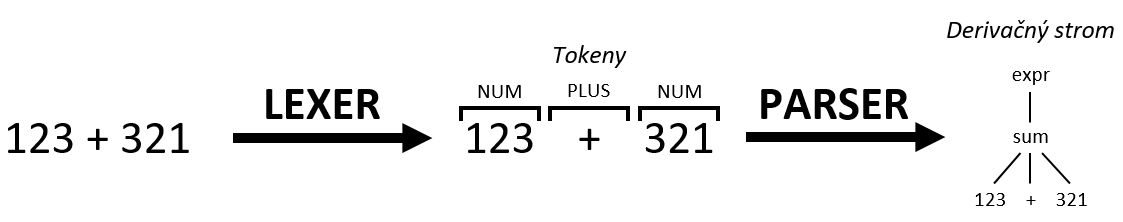
\includegraphics[width=14cm]{figures/lexer_parser.PNG}
\caption{Spracovanie reťazca \textit{123 + 321} lexerom a parserom}
\label{fig:lexer_parser}
\end{center}
\end{figure}

Pre príklad z obrázku \ref{fig:lexer_parser}  máme dva typy tokenov. \textbf{NUM} vyjadrujúci akékoľvek prirodzené číslo a \textbf{PLUS} vyjadrujúci znak súčtu (+). Keď sa lexer bude snažiť analyzovať reťazec \textbf{123 + 321}, bude čítať znaky \textit{1,2,3} a potom znak medzery. V tomto momente lexer rozpozná, že postupnosť znakov \textit{123} súhlasí z definíciou tokenu typu NUM. Následne prečíta znak \textit{+}, ktorý sa zhoduje s druhým typom tokenu PLUS a nakoniec objaví posledný token typu NUM. Takto definované tokeny použije parser na vyhodnotenie výsledného výrazu. Bezkontextová gramatika pre takýto parser by mohla vyzerať nasledovne:

\begin{center}
\begin{tabular}{p{0.35\textwidth}}
\textbf{sum} = NUM \{PLUS NUM\}
\end{tabular}
\end{center}

Vzhľadom na to, že lexery sú takmer výlučne používané v spojení s parsermi, je nutné si určiť hranicu, kde končí práca lexeru a kde začína práca parseru. Táto hranica nemusí byť vždy jasná a všetko to závisí na konkrétnej potrebe programu, pre ktorý je parser vytváraný. Pre príklad si môžeme predstaviť program, ktorý parsuje vstup obsahujúci IP adresu. Pokiaľ programu stačí poznať hodnotu IP adresy, tak je možné vytvoriť token v lexeru, ktorý popisuje celý formát IP adresy a parser pri svojej analýze použije iba tento token. 
\begin{center}
IPv4 = [0-9]+ "."\text{ [}0-9]+ "."\text{ [}0-9]+ "."\text{ [}0-9]+
\end{center}

Ak by bol problém zložitejší a program by chcel analyzovať IP adresu a zistiť z nej informácie, ako napríklad krajinu, bude parser potrebovať jednotlivé hodnoty IP adresy samostatne. V tomto prípade lexer rozdelí IP adresu na dva druhy tokenov (číslo a bodka).

\begin{center}
\begin{tabular}{p{0.65\textwidth}}
\color{editorGray}{/* Lexer */}\\
DOT   = "\text{.}"\\
OCTEC = [0-9]+\\
\color{editorGray}{/* Parser */}\\
ipv4  = OCTET DOT OCTET DOT OCTET DOT OCTET
\end{tabular}
\end{center}

\section{Typické problémy parsovania}
Pri definovaní gramatiky pre parsre existuje niekoľko typických problémov, s ktorými sa jednotlivé parsre musia vysporiadať. 

\subsection{Chýbajúci token}
Častým problémom v gramatikách sú chýbajúce resp. nedefinované tokeny. V niektorých gramatikách sa v rámci lexeru zadefinuje iba časť tokenov ako napríklad

\begin{center}
\begin{tabular}{p{0.3\textwidth}}
\color{editorGray}{/* Lexer */}\\
NAME = [a-zA-Z]+\\
\color{editorGray}{/* Parser */}\\
greeting = "Hello"{ NAME}
\end{tabular}
\end{center}

Token "Hello"{ }nie je pre parser definovaný. Niektoré nástroje na parsovanie sa dokážu s týmto problémom vysporiadať tým, že si sami vygenerujú definíciu pre tieto tokeny, čím zároveň ušetria užívateľovi trochu času \cite{tomassetti:parsing}.

\subsection{Pravidlá s ľavou rekurziou}\label{left-recursion-rule}
V rámci bezkontextových gramatík sa často využíva ľavá rekurzia na definovanie zľava asociatívnych operácií. Tento problém sa najčastejšie rieši v rámci Top Down parserov (viď kapitola \ref{parsing-alg-basics}) s rekurzívnym zostupom (viď kapitola \ref{recursive-descent}). 

Pravidlá s ľavou rekurziou sú také pravidlá, ktoré začínajú s referenciou samy na seba, ako napríklad $A \rightarrow A\alpha$. Do toho problému spadá taktiež nepriama ľavá rekurzia, čo znamená že referencia na samého seba sa objaví v rámci iného pravidla, ako napríklad:

\begin{center}
\begin{tabular}{p{0.15\textwidth}}
$A \rightarrow B\alpha$\\
$B \rightarrow A\beta$\\
\end{tabular}
\end{center}

Predpokladajme, že sa snažím zparsovať pravidlo $A$ na danom mieste vo vstupnom reťazci. Ak by sme na to použili Top Down parser, ktorý pracuje z ľava do prava, našou prvou podúlohou by bolo parsovať pravidlo $A$ na tom istom mieste \cite{moore2000removing}. Takto sa okamžite dostávame do nekonečnej slučky. Rovnaký problém nastane aj s použitím gramatiky, ktorá obsahuje nepriamu ľavú rekurziu, kde sa do nekonečnej slučky dostaneme prechodom cez viac pravidiel.

V teórii, obmedzenie na bezkontextové gramatiky bez ľavej rekurzie nepridáva žiadne obmedzenie na jazyk, ktorý sa snažíme popísať gramatikou. Existujú pravidlá, pomocou ktorých sa dá ľavá rekurzia odstrániť. V zásade každá bezkontextová gramatika obsahujúca ľavú rekurziu môže byť transformovaná na gramatiku bez ľavej rekurzie \cite{moore2000removing}.

% \textbf{Note: moznost pridat priklad odstranovania lavej rekurzie}
% https://tomassetti.me/guide-parsing-algorithms-terminology/#typicalGrammarIssues
